\documentclass[]{article}
\usepackage{amsmath,graphicx}

\newcommand{\beq}{\begin{equation}}
\newcommand{\eeq}{\end{equation}}
\newcommand{\Tsys}{T_\text{sys}}
\newcommand{\kv}{\mathbf{k}}

\begin{document}

\title{HERA Sensitivity Calculation}
\author{Josh Dillon}
\date{\today} 
\maketitle


\section{Purpose of this calculation}
The purpose of this calculation is to predict the sensitivity of HERA for a range of sizes and assumptions about foreground mitigation strategy.  Since there's been a lot of confusion about the calculation of noise for HERA, I would like to translate the power spectrum derivation from Parsons et al. (2012a; P12a) into the language of covariance matrices and quadratic estimators of Liu \& Tegmark (2011) and Dillon et al. (2013a; D13a).

\section{Assumptions}
Here's a list of the assumptions that go into the calculation.  I'll try to be as detailed as possible, since it's very easy to equivocate here.
\begin{itemize}
\item The array is a hexagonal number (37, 127, 331, or 547) of 14 meter diameter dishes with maximally dense (hexagonal) packing.  The array is at latitude $-30^\circ$.
\item The primary beam has a FWHM of $9.8^\circ \times (150\mbox{ MHz} / \nu)$.
\item For the purposes of calculating $\Omega_p$, $\Omega_{pp}$, and $\Omega'$, I assume the beam is a Gaussian.  For simplicity, I assume each field (the mapped region) is square and that the sky is approximately flat on these angular scales.
\item I consider 9 independent fields of $9.8^\circ \times 9.8^\circ$ each, spanning the EoR cold spot's 6 hours of RA.  
\item The data cube for each field has an 8 MHz bandwidth and a 100/1024 MHz frequency resolution.  Matching the pixel size to the synthesized beam, this yields a $38 \times 38 \times 80$ voxel data cube for each field with a volume of $1550 \times 1550 \times 137$ Mpc$^3$.
\item I assume one year of continuous nighttime observation.  Each field gets $365 \times 12 \times (9.8^\circ / 360^\circ) = 119$ hours of observation.
\item I'm assuming a system temperature $T_\text{sys} = T_\text{rec} + T_\text{sky}$ with $T_\text{rec} = 100 \mbox{ K}$ (consistent with PAPER) and $T_\text{sky} = 60 \mbox{ K} \times (\lambda / 1\mbox{ m})^{2.55}$, following Bergman (1999), the fiducial value that LOFAR uses.
\item I'm assuming that the power spectrum from each field can be averaged together and that the uncertainty on the power spectrum scales as $1/\sqrt{N_\text{fields}}$.
\item I'm assuming a fiducial power spectrum $\bar{x}_{HI} = 0.5$ Lidz, following Parsons et al. (2013; P13).  I'm assuming that cosmic variance errors can be added in quadrature to noise errors and that they do not affect window functions (this is not true, but also not very important).
\item For simplicity, each scalar $k$ bin is the weighted average of all $k_\perp$ bins for a given value of $k_\|$.  See Figure \ref{fig:BinningDiagram}.
\begin{figure*} [!ht] 
	\centering 
	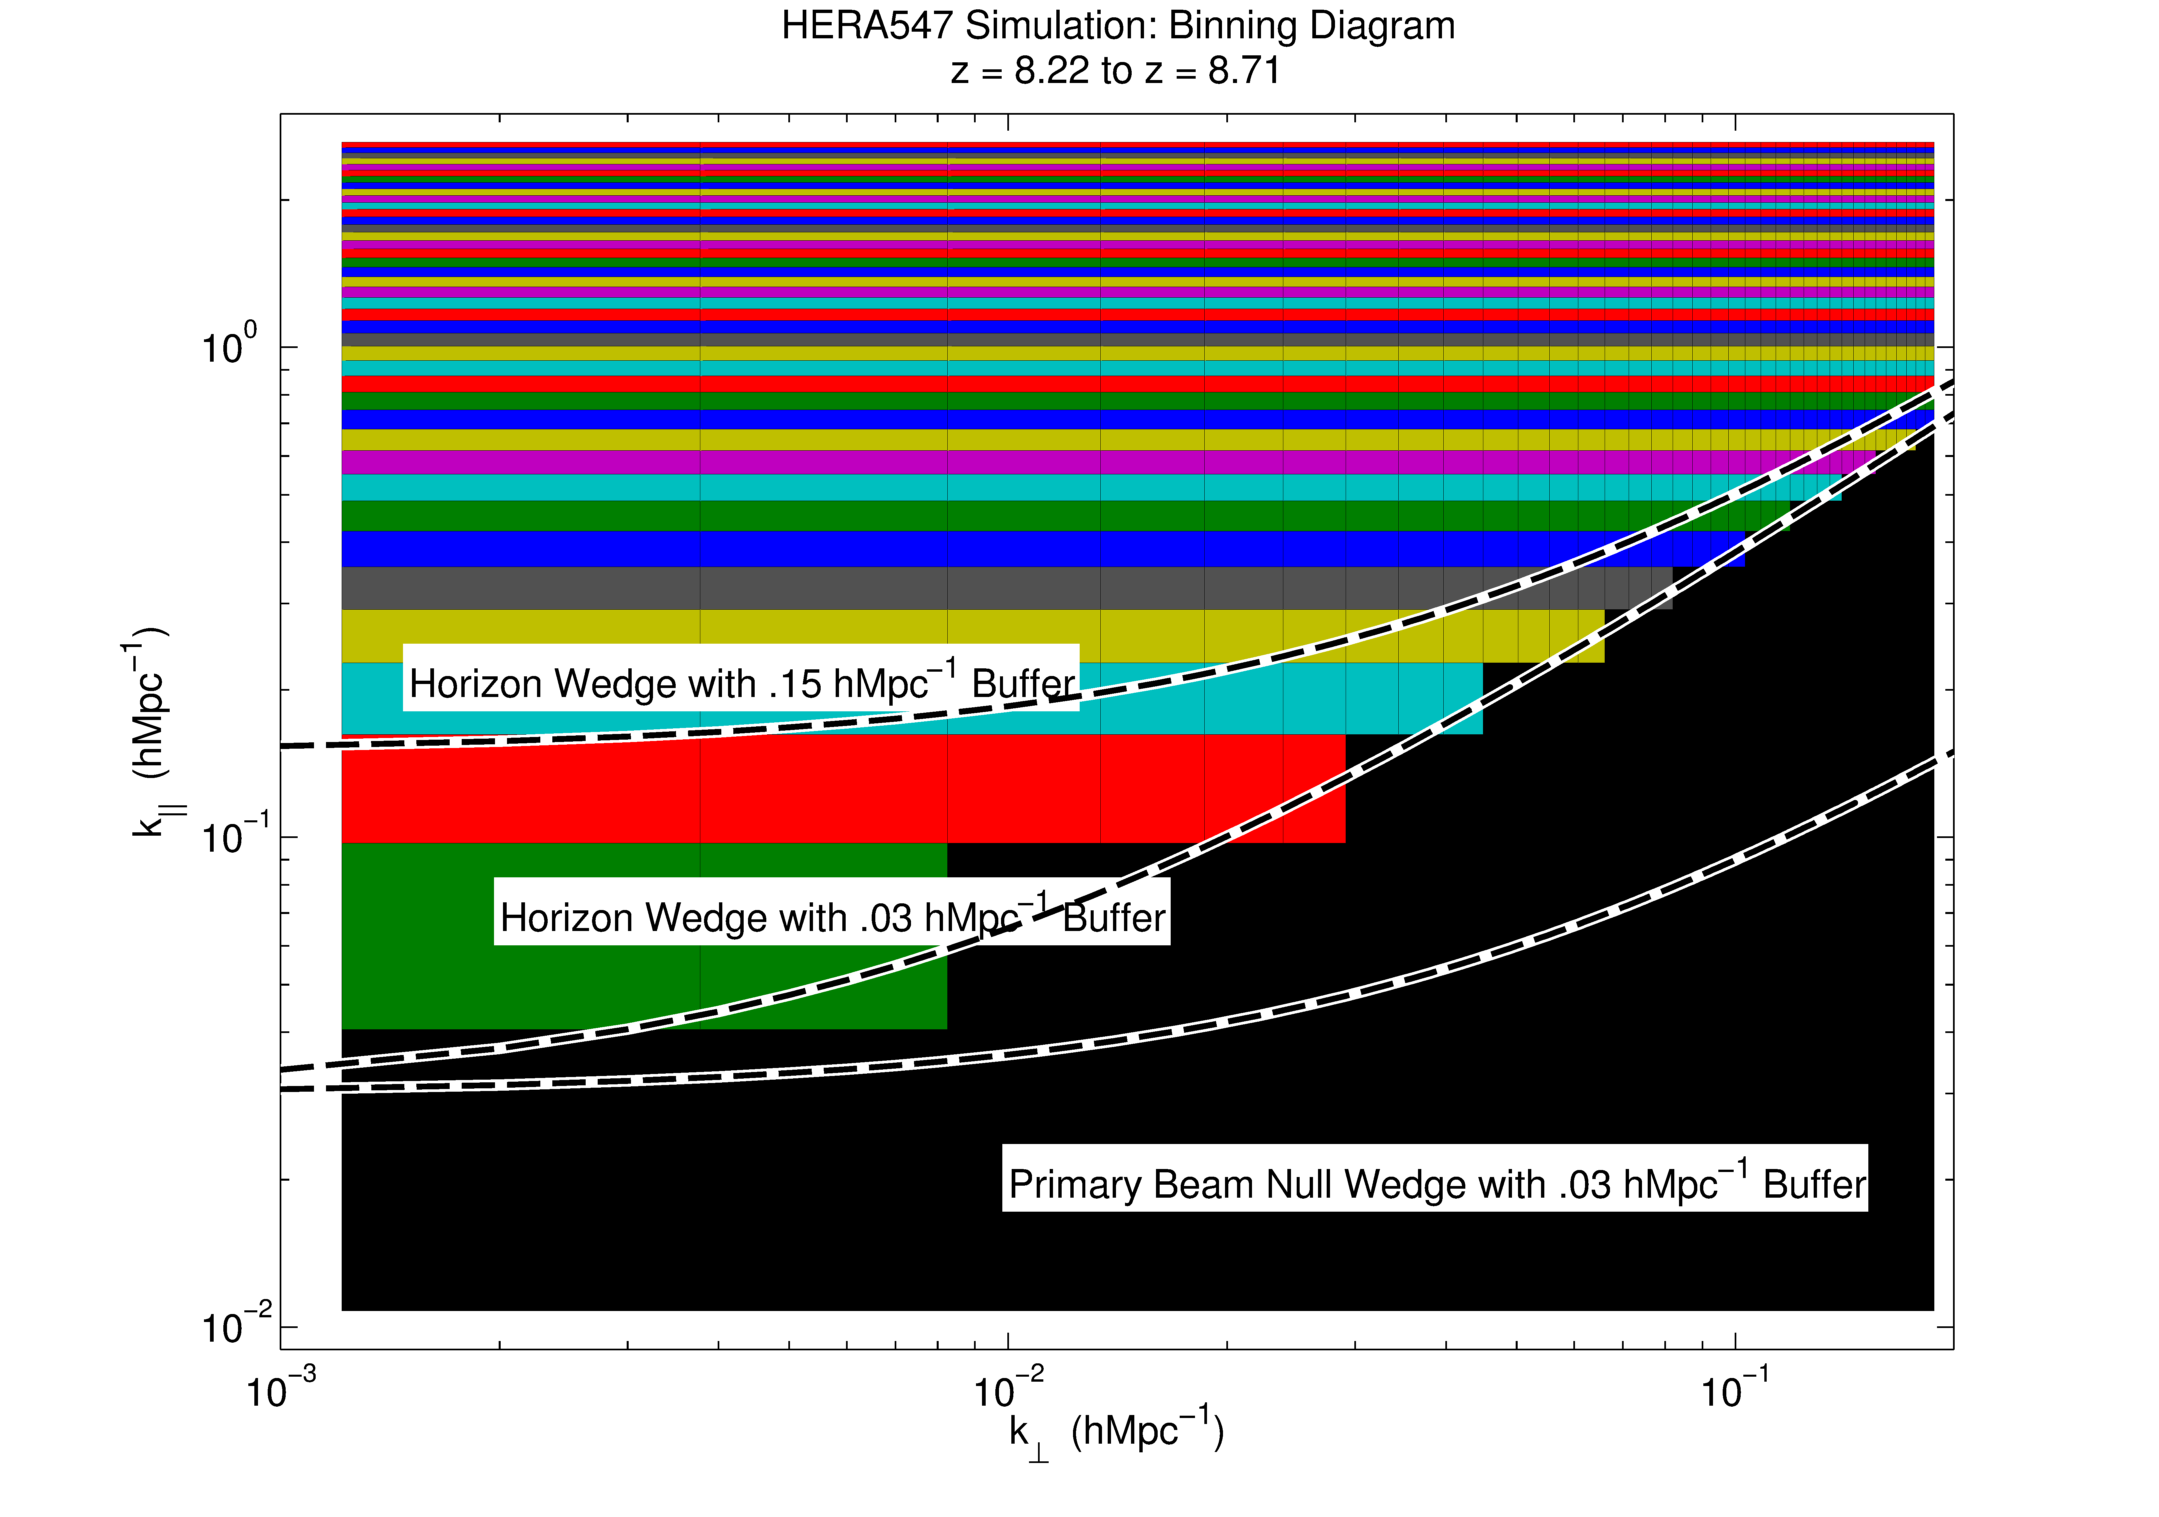
\includegraphics[width=1\textwidth]{Binning.png}
	\caption{Example bins (each color is a different $k$ bin) for the ``fiducial" choice of foreground excision, with all three foreground regions shown.}
	\label{fig:BinningDiagram}
\end{figure*} 
\item To approximate a more precise method of foreground mitigation, I excise a region of cylindrical $k$ space corresponding to
\begin{equation} k_\| \le \left[ \sin \theta \frac{D_M (z) E(z)}{D_H (1+z)} \right] k_\perp + \text{Buffer} \end{equation}
where $D_H \equiv c/H_0$, $E(z) \equiv \sqrt{\Omega_m (1+z)^3 + \Omega_\Lambda}$, $D_M(z) \equiv \int_0^z dz^\prime / E(z^\prime)$, and $\theta$ is angular radius of the the field-of-view. I consider three cases:
\begin{enumerate}
\item A ``conservative" case where $\theta = 90^\circ$ (the horizon) and the buffer is 0.15 $h^{-1}$ Mpc.
\item A ``fiducial" or mid-range case" where $\theta = 90^\circ$ and the buffer is 0.03 $h^{-1}$ Mpc.
\item An ``optimistic" case matching Beardsley et al. (2012) where $\theta = 13.15^\circ \times (150\mbox{ MHz} / \nu)$, the first primary beam null, and the buffer is 0.03 $h^{-1}$ Mpc.
\end{enumerate}
See Figure \ref{fig:BinningDiagram} for what these three cuts look like.
\end{itemize}


\section{Results}
In Figures \ref{fig:ArrayComp} and \ref{fig:ForegroundComp}, I compare the sensitivity for all four stages of HERA and for all three foreground mitigation strategies outlined above.

\begin{figure*} [!ht] 
	\centering 
	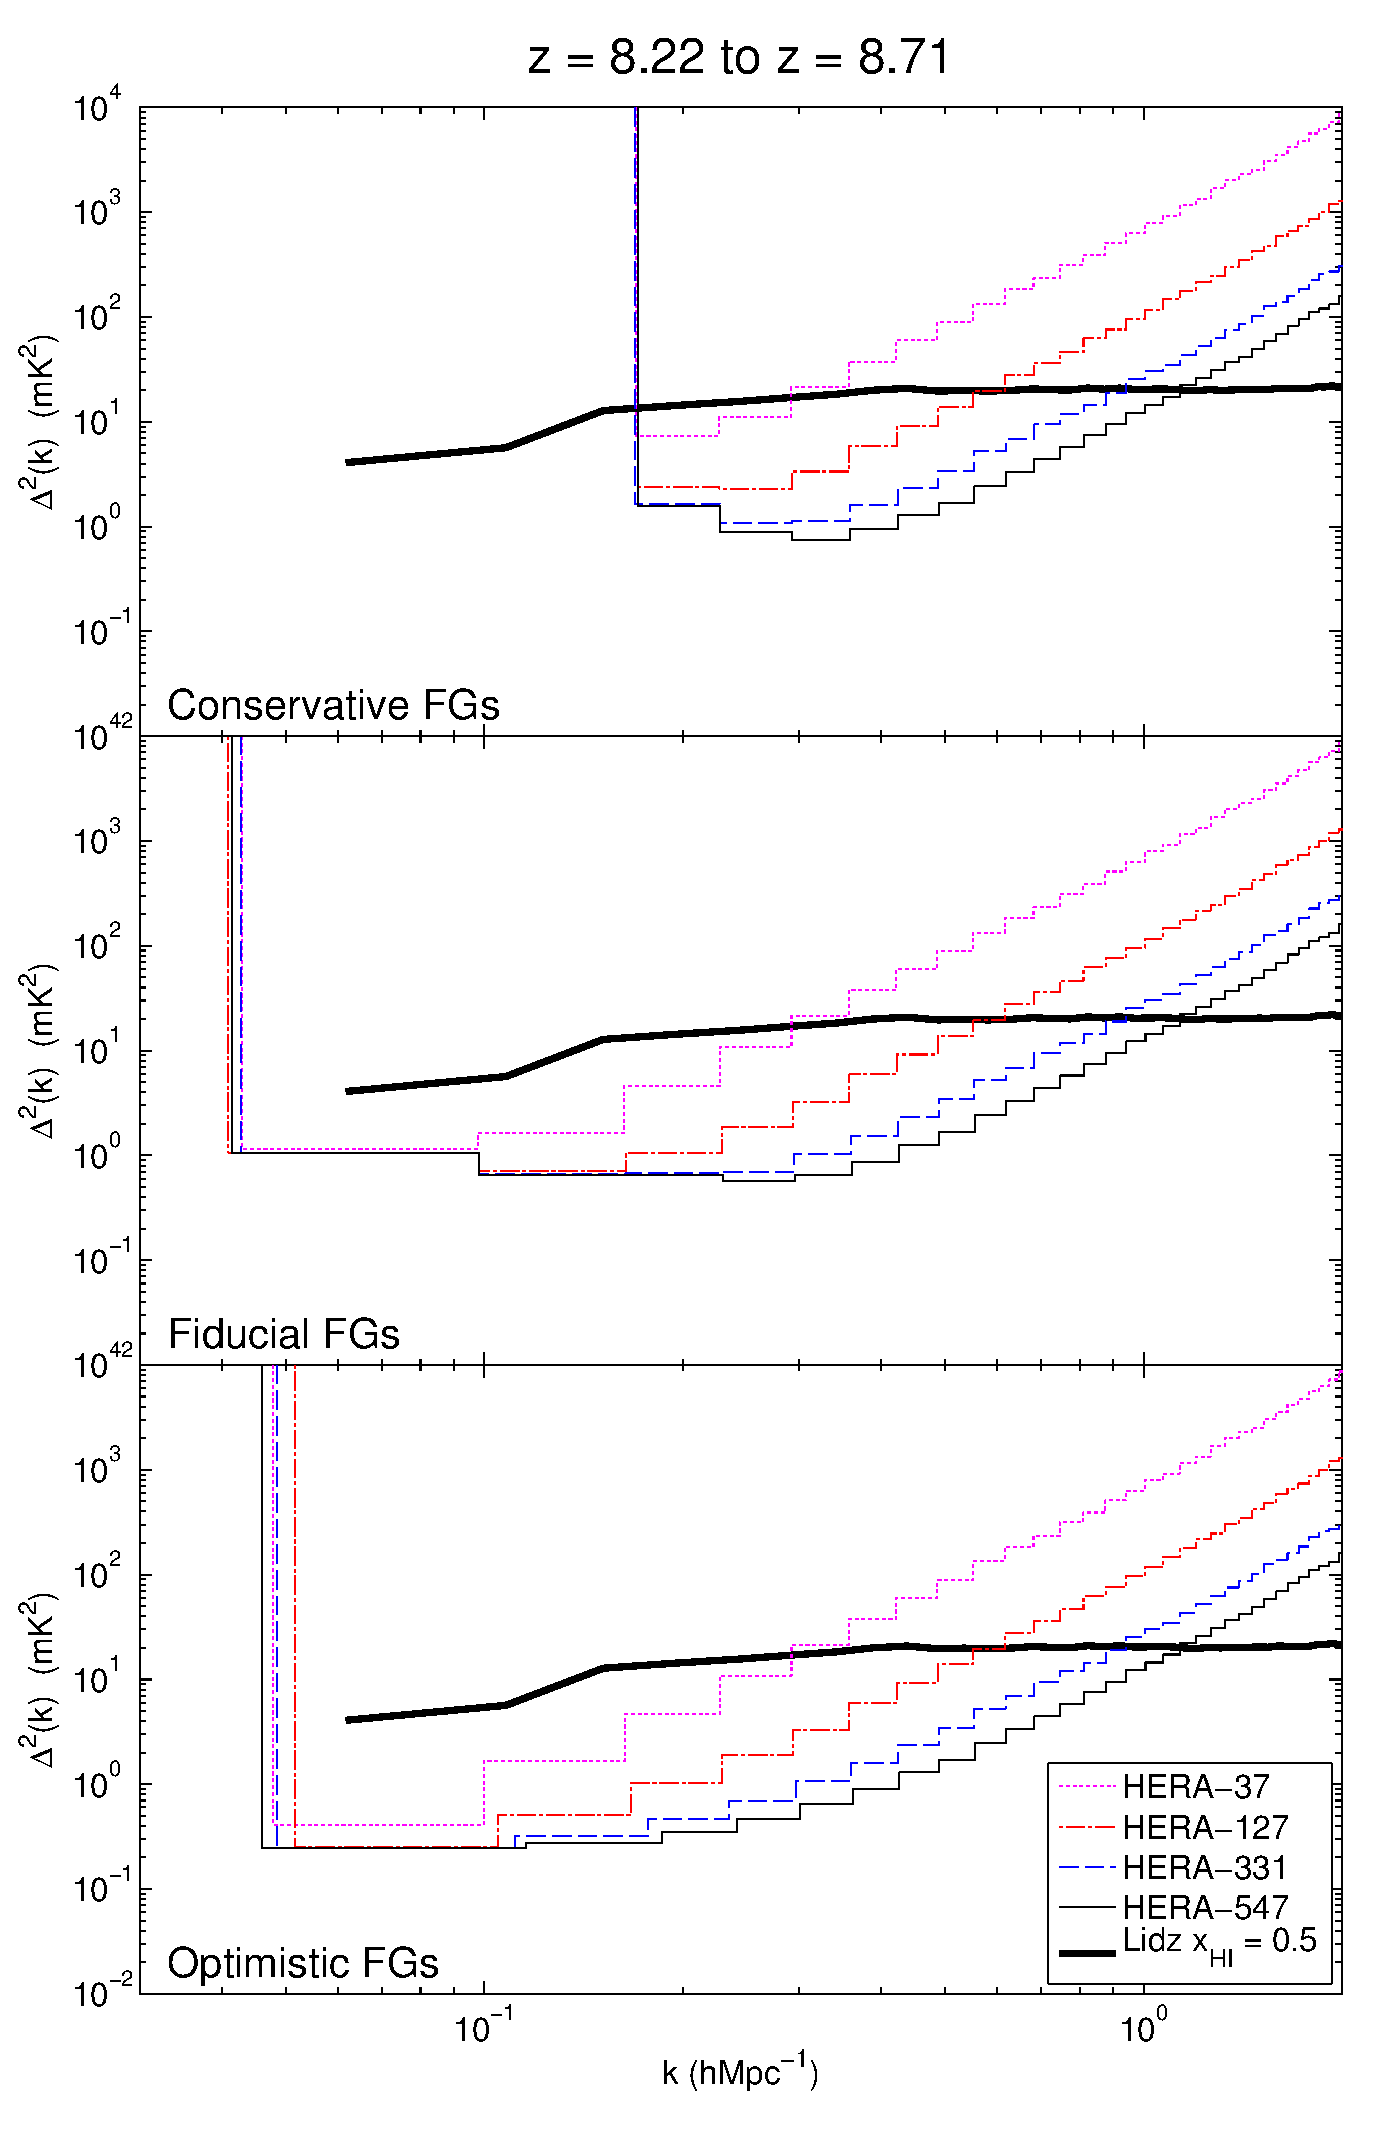
\includegraphics[width=.6\textwidth]{HERA_Array_Comp.pdf}
	\caption{Comparing the performance of different HERA arrrays for three different levels of foreround excision.}
	\label{fig:ArrayComp}
\end{figure*} 

\begin{figure*} [!ht] 
	\centering 
	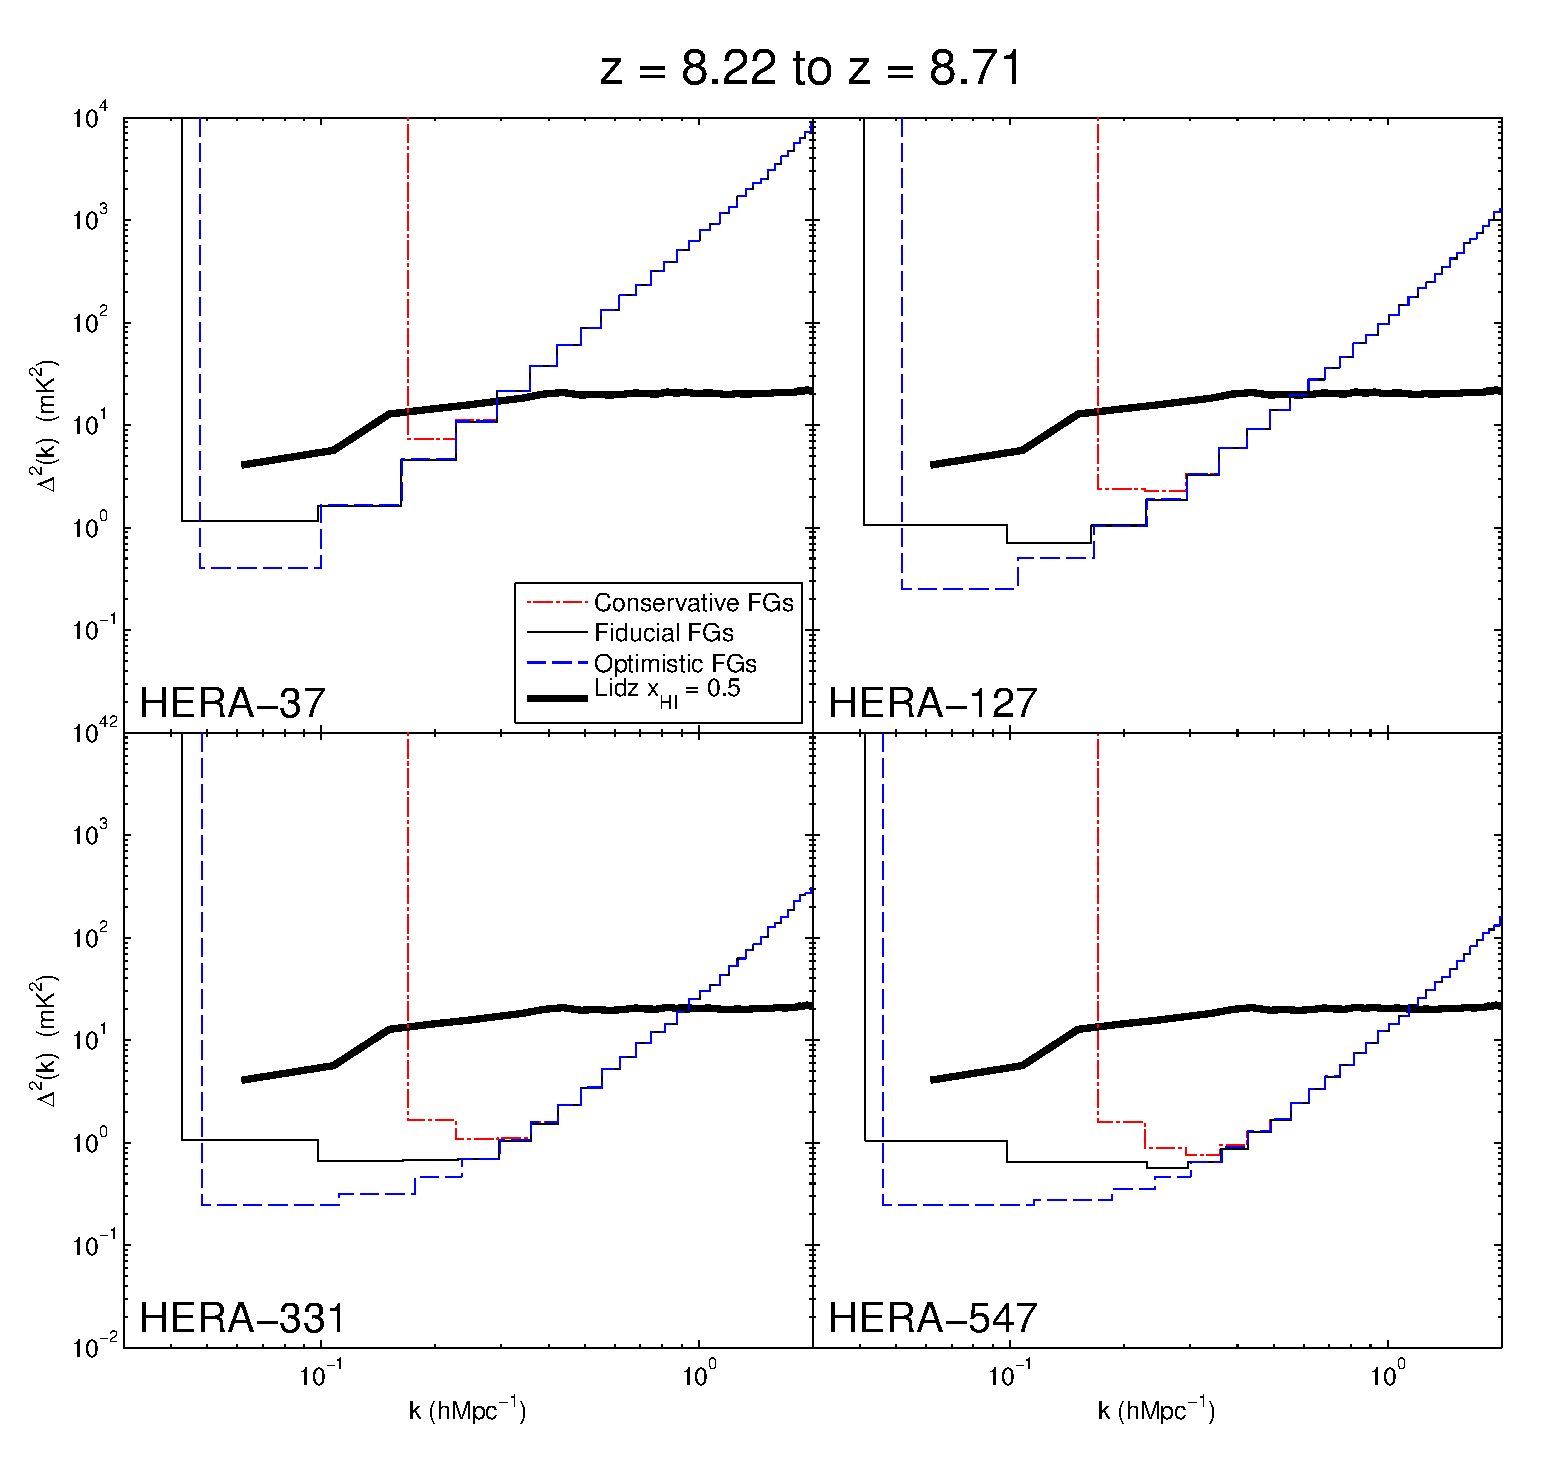
\includegraphics[width=1\textwidth]{HERA_Foreground_Comp.pdf}
	\caption{Same data as in Figure \ref{fig:ArrayComp}, plotted a different way.  This compares the effect of foreground excision on each of the four HERA stages.}
	\label{fig:ForegroundComp}
\end{figure*}


The profound difference that the foreground cut has is attributable to the noise structure of $\Delta^2(k)$ in cylindrical Fourier space.  See Figure \ref{fig:CylDeltaSq}.
\begin{figure*} [!ht] 
	\centering 
	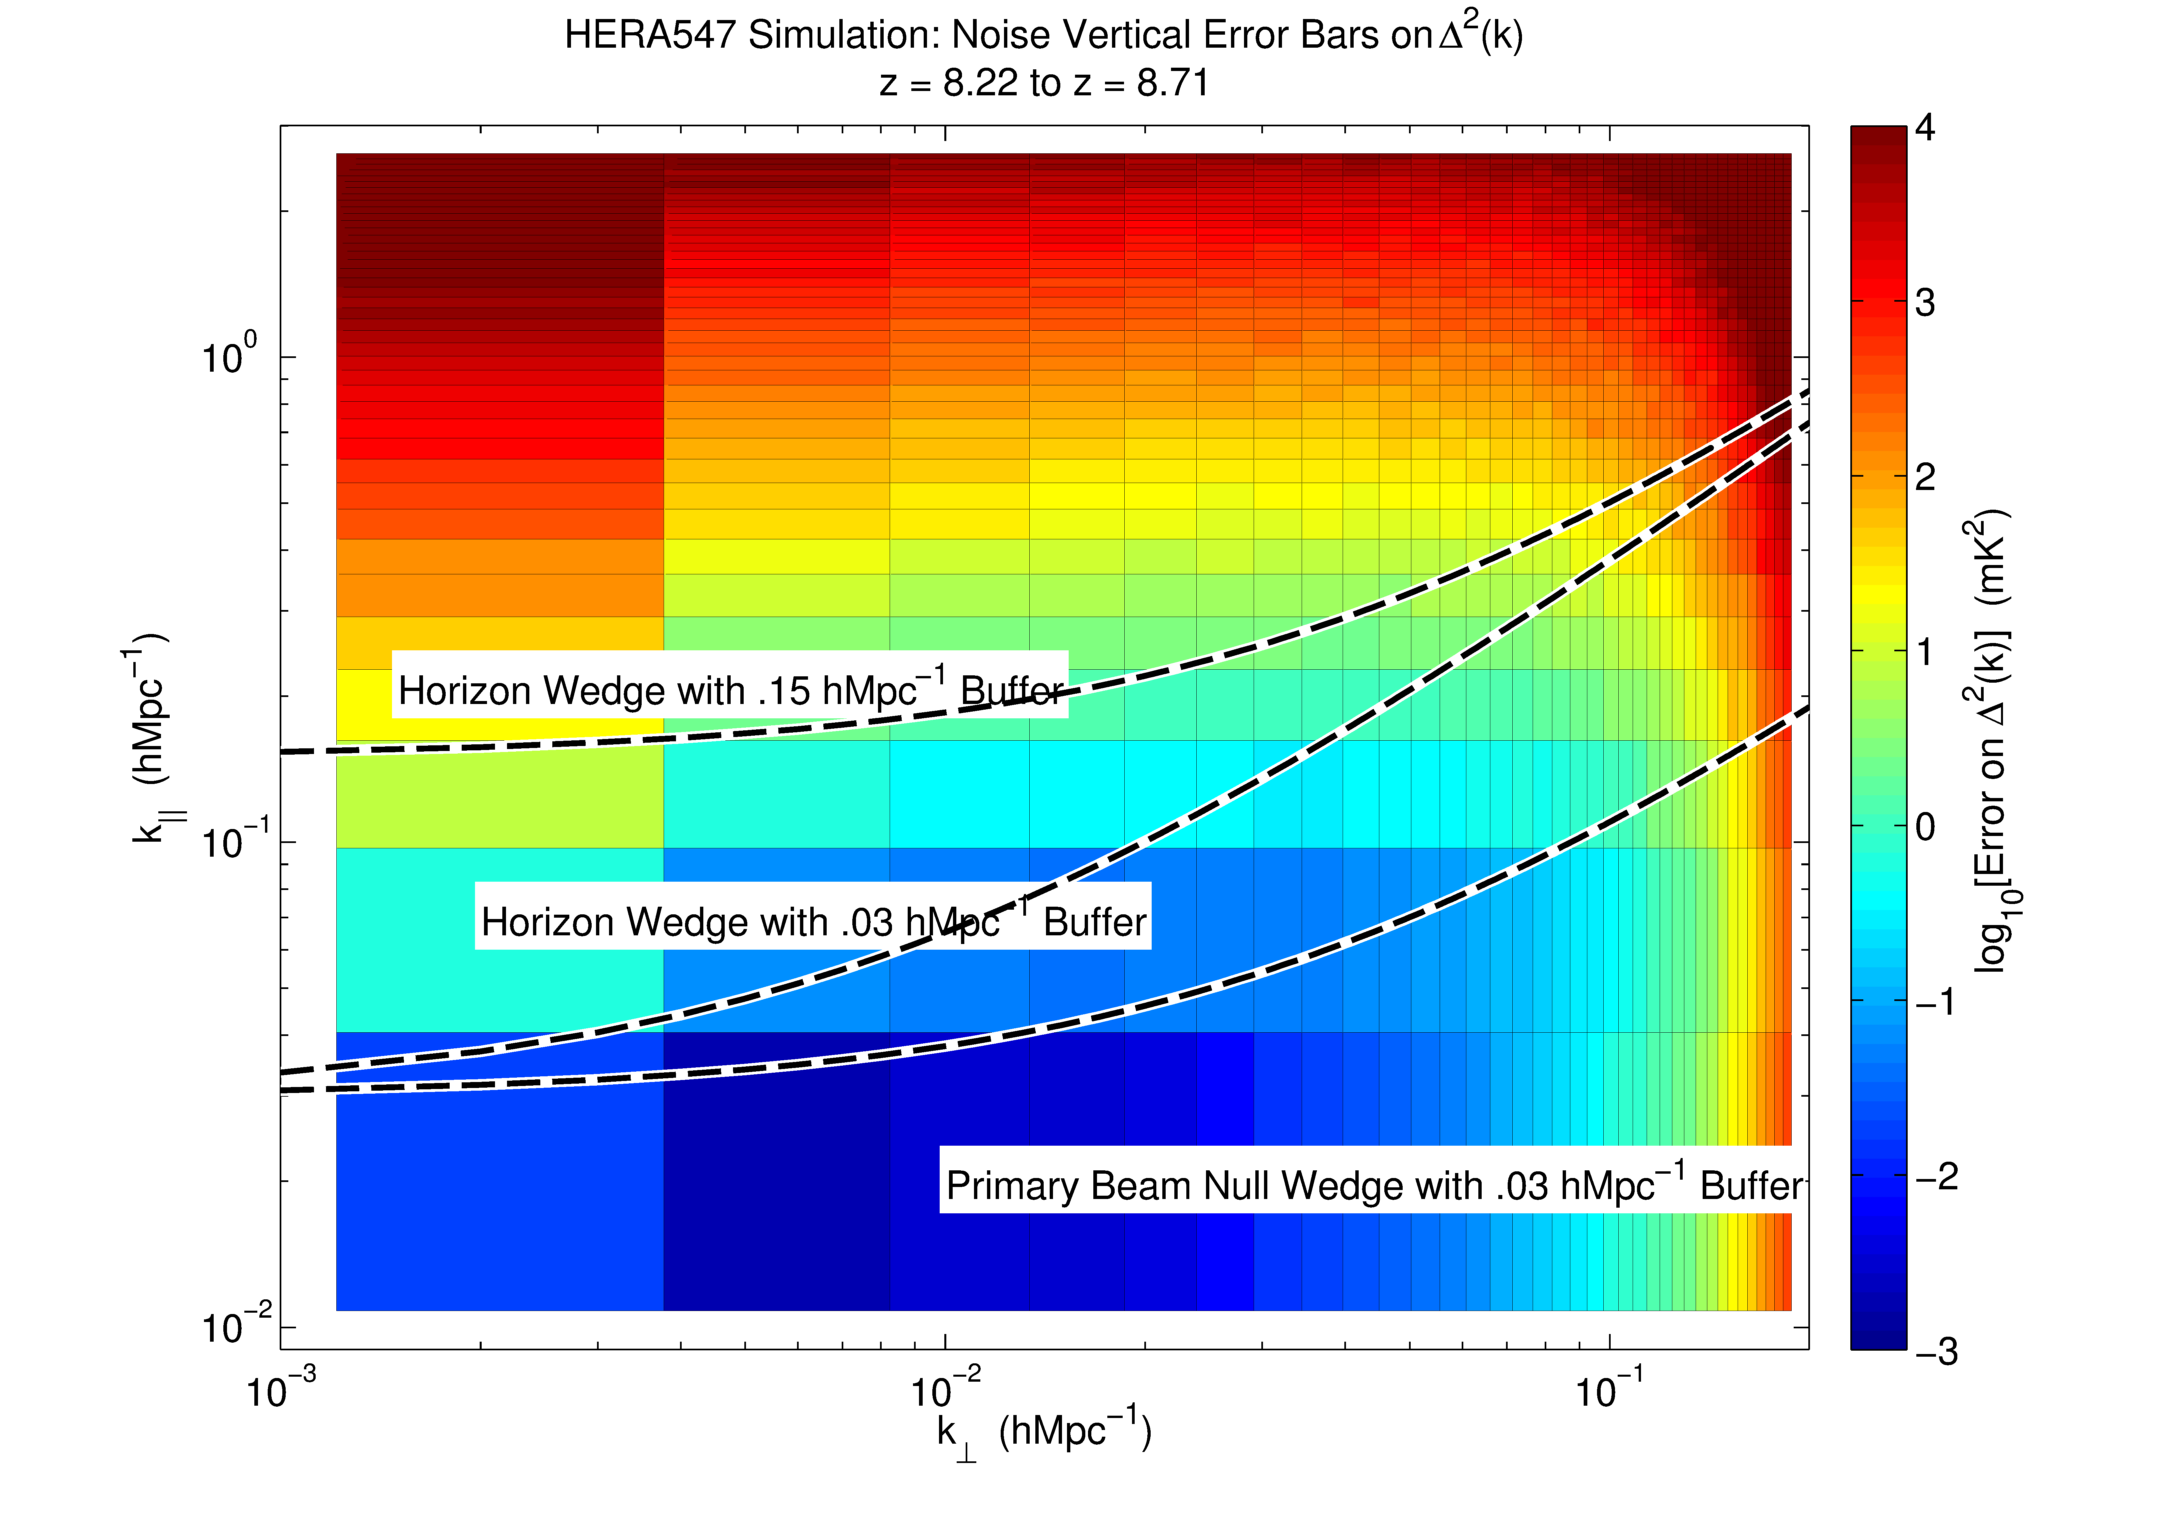
\includegraphics[width=1\textwidth]{CylDeltaSqError.png}
	\caption{Cylindrical $\Delta^2(k)$ errors show why the foreground cut matters so much.}
	\label{fig:CylDeltaSq}
\end{figure*} 


\section{Detailed calculation}



The point of this calculation is to connect the noise power spectrum language of P12a with the covariance matrix language of D13a. According to P12a,\footnote{The 4 in the denominator of \eqref{DimensionlessNoisePS} is a 2 in P12a, but should have been a 4 to account for two polarizations.}
\beq
\Delta^2_N(\kv) = X^2 Y \frac{k^3}{2\pi^2}\frac{\Omega}{4t(\kv)}\Tsys^2 \label{DimensionlessNoisePS}.
\eeq
Furthermore, P13 argues that $\Omega$ in \eqref{DimensionlessNoisePS} should have been replaced by $\Omega' \equiv \Omega_p^2 / \Omega_{pp}$ where
\beq
\Omega_{pp} \equiv \int dl dm |A(l,m)|^2
\eeq
and 
\beq
\Omega_{p} \equiv \int dl dm A(l,m).
\eeq

So, how do we convert this this into the language of covariance matrices? Well, from \eqref{DimensionlessNoisePS}, we can go back to a dimensionful power spectrum
\beq
P^N(\kv) = X^2 Y \frac{\Omega'}{2t(\kv)}\Tsys^2.
\eeq  
The noise covariance between real space voxels $i$ and $j$ is related to the power spectrum by
\beq
C^N_{ij} = \int \widetilde{\psi}_i(\kv)\widetilde{\psi}^*_j(\kv) P^N(\kv)\frac{d^3k}{(2\pi)^3}.
\eeq
$\widetilde{\psi}_i(\kv)$ is the Fourier transform of the real-space pixelization function for the $i$th pixel.  In previous work, I have used a boxcar pixelization function, which introduces a $j_0$ function.  In this calculation, I'm assuming a boxcar function in 2D Fourier space, since the pixelization of $P^N(\kv)$ is fundamentally in the $uv$-plane.

The integral over $k_z$ is trivial because the noise must be uncorrelated between frequencies.  Though the integrand has a frequency dependence, the  derivation of $\Delta_N^2(\kv)$ in \eqref{DimensionlessNoisePS} actually depends on ignoring that dependence.  So, without any loss of generality (actually, I think there's a gain in generality by undoing that assumption),
\beq
C^N_{ij} = \frac{\delta_{\nu_i \nu_j}}{Y\Delta \nu} \int e^{i k_x (x_i - x_j)} e^{i k_y(y_i-y_j)} X^2 Y \frac{\Omega'}{2t(u,v,\lambda)}\Tsys^2 \frac{dk_x dk_y}{(2\pi)^2},
\eeq
where $\Delta \nu$ is the frequency resolution of the instrument and where I've folded all pixelization into $t(k_x,k_y,\lambda)$, which I am assuming is piecewise constant for each frequency and each $uv$-cell.  Because of that, we can rewrite the integral as a sum over all $k_x$ and $k_x$ (or equivalently, all $u$ and $v$):
\beq
C^N_{ij} = \frac{\delta_{\nu_i \nu_j}}{Y \Delta \nu}\sum \frac{2\pi}{L_x}  \frac{2\pi}{L_y} \frac{1}{(2\pi)^2} e^{i k_x (x_i - x_j)} e^{i k_y(y_i-y_j)} X^2 Y \frac{\Omega'}{2t(u,v,\lambda)}\Tsys^2
\eeq
where $L_x$ is the comoving size of the data cube I'm considering.  For now, let's consider a data cube the size of the primary beam,\footnote{Something subtle happens when considering the noise in a facet of the primary beam, which I've been thinking about and which will be relevant when comparing MWA and PAPER sensitivities to HERA...a topic for later.} meaning that $L_x L_y = \Omega_p X^2$.  Following the trick of creating new Kronecker deltas in Equation (B9) of D13a, 
we can write $\mathbf{C}^N$ as 
\beq
\mathbf{C}^N \equiv \mathbf{F}^\dagger_\perp \widetilde{\mathbf{N}} \mathbf{F}_\perp
\eeq
where $\mathbf{F}_\perp$ and $\mathbf{F}^\dagger_\perp$ are discrete, unitary 2D (inverse) Fourier transform matrices (introducing a factor of $n_x n_y$, the number of pixels in the data cube perpendicular to the line of sight).
\begin{align}
\widetilde{N}_{ij} &= \frac{\delta_{ij}}{Y\Delta \nu} \frac{n_x n_y X^2 Y}{\Omega_p X^2} \frac{\Omega'}{2t(u_i,v_i,\lambda_i)}\Tsys^2 \\
&=\frac{\delta_{ij}\Tsys^2\Omega'}{2 t(u_i,v_i,\lambda_i) \Delta \nu \Omega_\text{pix}} , \label{Nfourier}
\end{align}
since $\Omega_p / n_x n_y = \Omega_\text{pix}$, the angular size of each real space pixel.

From here, the calculation of the error on $\Delta^2(k)$ proceeds as it does in Dillon et al. (2013b), with $\mathbf{M} \propto \mathbf{F}^{-1/2}$.  However, this sensitivity assumes that we measure an auto-power spectrum, not a cross power spectrum between independent observations separated in time.\footnote{Additionally, unlike in that work, the sample variance error is added to the final vertical error bars in quadrature at the very end, rather than going through the whole quadratic estimator framework.  Implementing that correctly is another task for later.}

\end{document}